%!TEX root = ../main.tex

\subsection{The Windowing Heuristic}\label{app:delta-heuristic-exps}

\begin{figure}
	\centering
	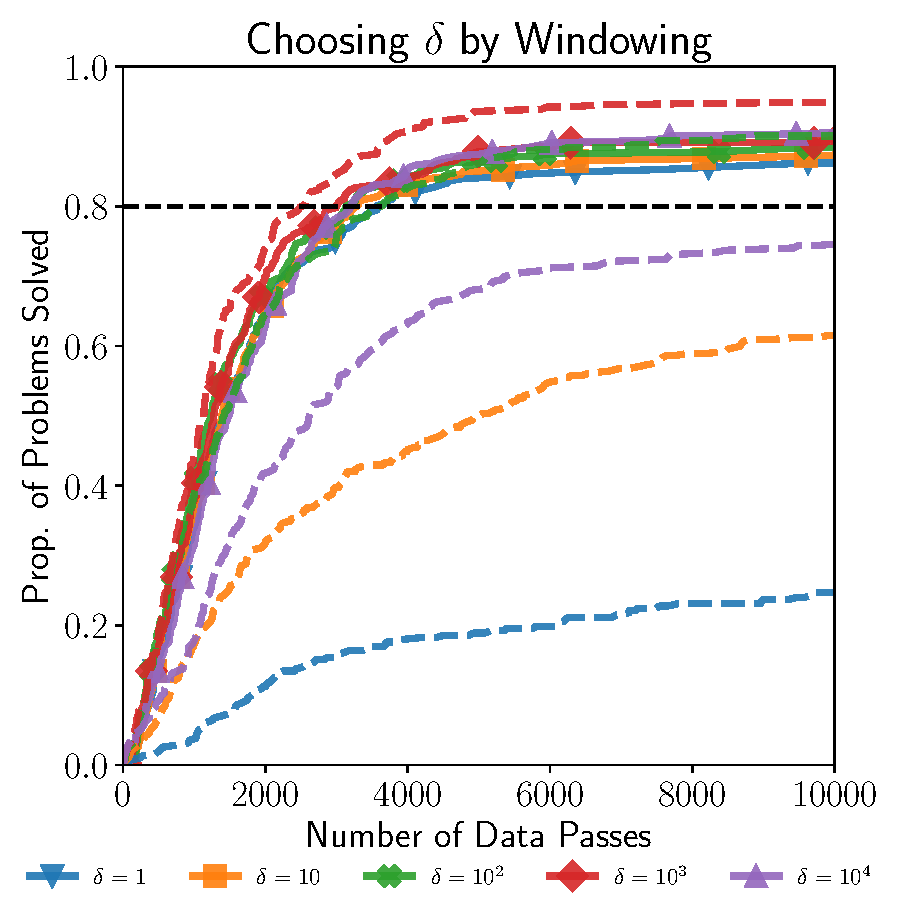
\includegraphics[width=0.95\linewidth]{figures/chapter_two/pp_delta.pdf}
	\caption{Performance profile comparing our AL method with (solid lines with markers) and without (dashed lines) the windowing heuristic for setting the penalty strength.
		We consider a wide range of initial \( \delta \) values and generate the profile by solving the C-ReLU problem on 73 datasets from the UCI repository with \( 6 \) different regularization parameters for each dataset.
		The windowing heuristic performs nearly as well as the best fixed \( \delta \) and without a noticeable computational overhead.
		In contrast, extreme values of \( \delta \) can cause the ``fixed'' approach to fail on approximately \( 40\% \) of problems.
	}%
	\label{fig:delta-pp}
\end{figure}

Recall that the key hyper-parameter for our AL method is the penalty strength, denoted \( \delta \).
Here we verify the effectiveness of the windowing heuristic for selecting \( \delta \) as proposed in Section~\ref{sec:reliable-co}.
Experimentally, the rule performs nearly as well as the best fixed value of \( \delta \) across a wide range of datasets and avoids the catastrophic failures which can occur when \( \delta \) is miss-specified.

We initialize our AL method with \( \delta_0 \in \cbr{1, 10, 10^2, 10^3, 10^4} \) and compare tuning \( \delta \) using the windowing heuristic against keeping \( \delta \) fixed throughout optimization.
All other parameters are identical and constant for the two approaches (see Appendix~\ref{app:default-parameters} for specifics).
To evaluate speed and robustness, we use another performance profile on the 438 problems generated from the UCI datasets as detailed in Appendix~\ref{app:uci-datasets}.
In this case, a problem is considered ``solved'' when the minimum-norm subgradient of the augmented Lagrangian is smaller than \( 10^{-3} \) and the norm of the constraint gaps is also less than \( 10^{-3} \).
This isn't equivalent to terminating when the Lagrangian function is approximately stationary, but we found the rule to work well in practice.
We use \( 500 \) randomly sampled activation patterns for the C-ReLU model.

\cref{fig:delta-pp} plots the result, with dotted lines for the AL method with fixed \( \delta \) and solid lines with markers for methods using the windowing heuristic.
Empirically, the windowing heuristic is nearly effective as the best fixed \( \delta \) and avoids the complete failure of AL methods with fixed, poorly specified penalty parameters (e.g. \( \delta = 1  \) or \( \delta = 10^4 \)).
Moreover, this is achieved at almost no overhead in terms of total data passes required for convergence.
Finally, we observe that fixing \( \delta = 10^3 \) works very well across all problems;
this is likely because the problems are carefully normalized before optimization to ensure they are on the same scale.
Specifically, the columns of the data matrix for each problem are unitized (Appendix~\ref{app:data-normalization}), and the augmented Lagrangian \( \calL_\delta \) is normalized by \( n * k \), where \( k \) is the number of classes.

\begin{figure}
	\centering
	\ifdefined\smallPDF
		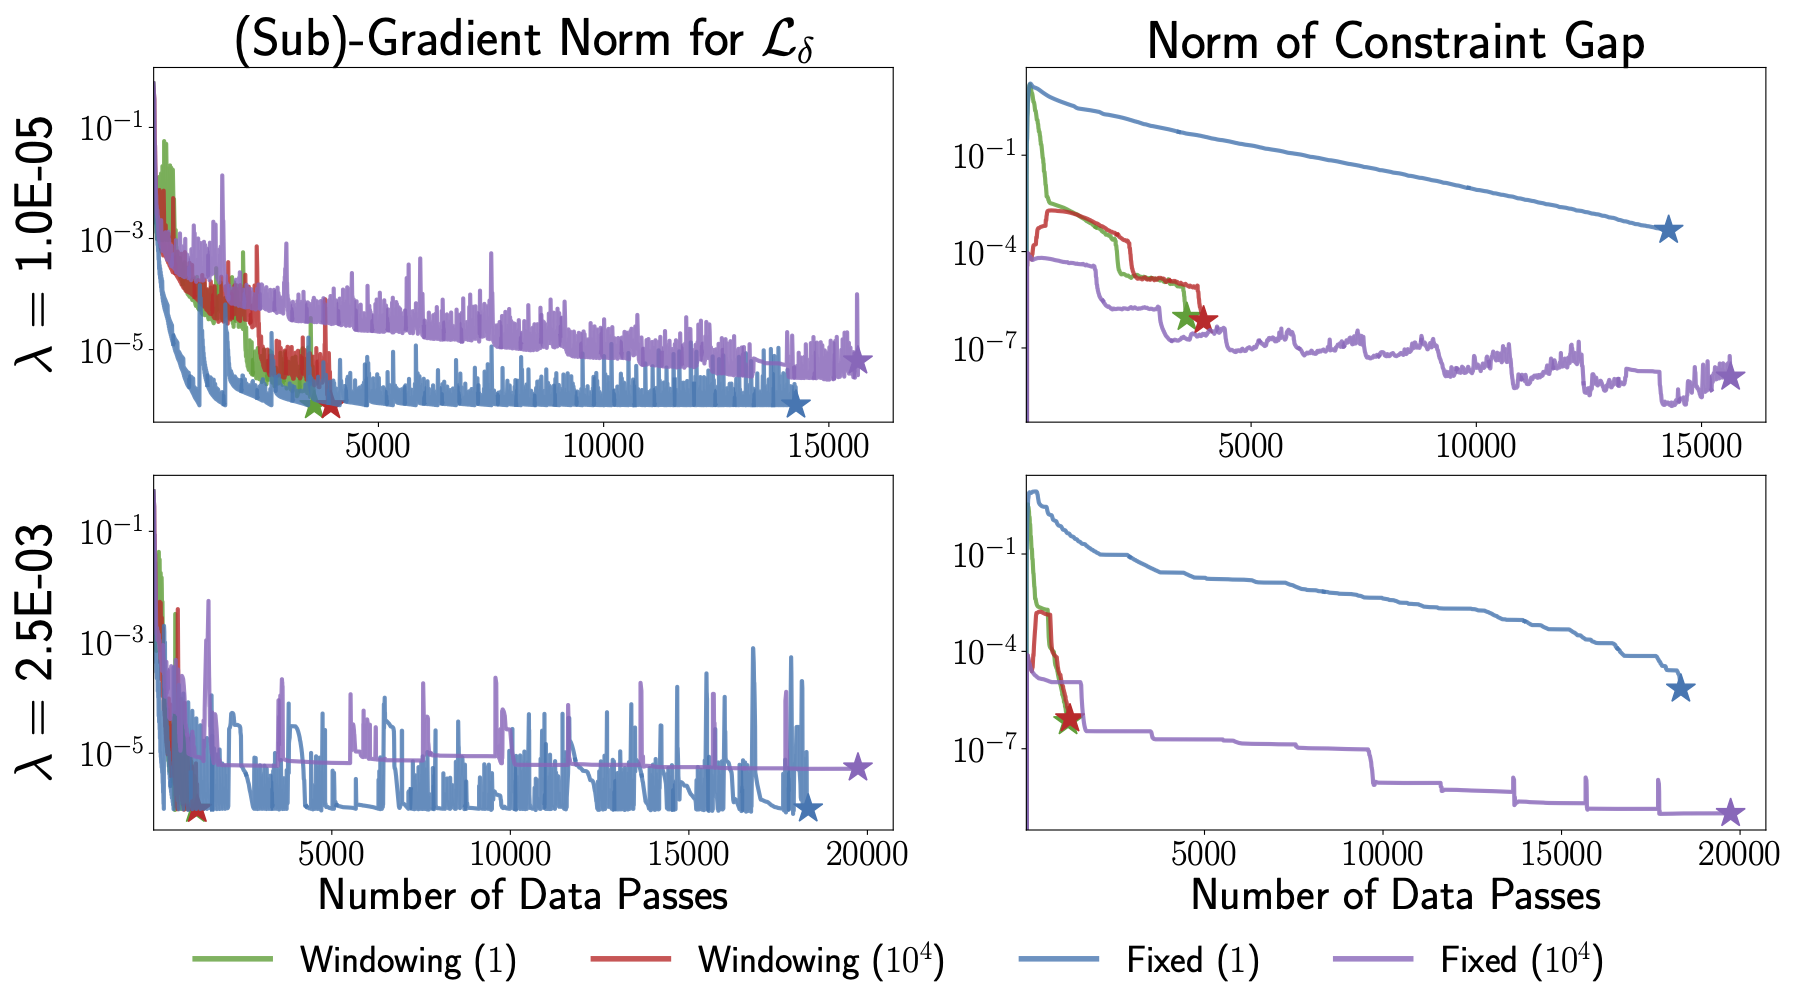
\includegraphics[width=0.95\linewidth]{figures/chapter_two/delta_heuristic/monks-2.png}
	\else
		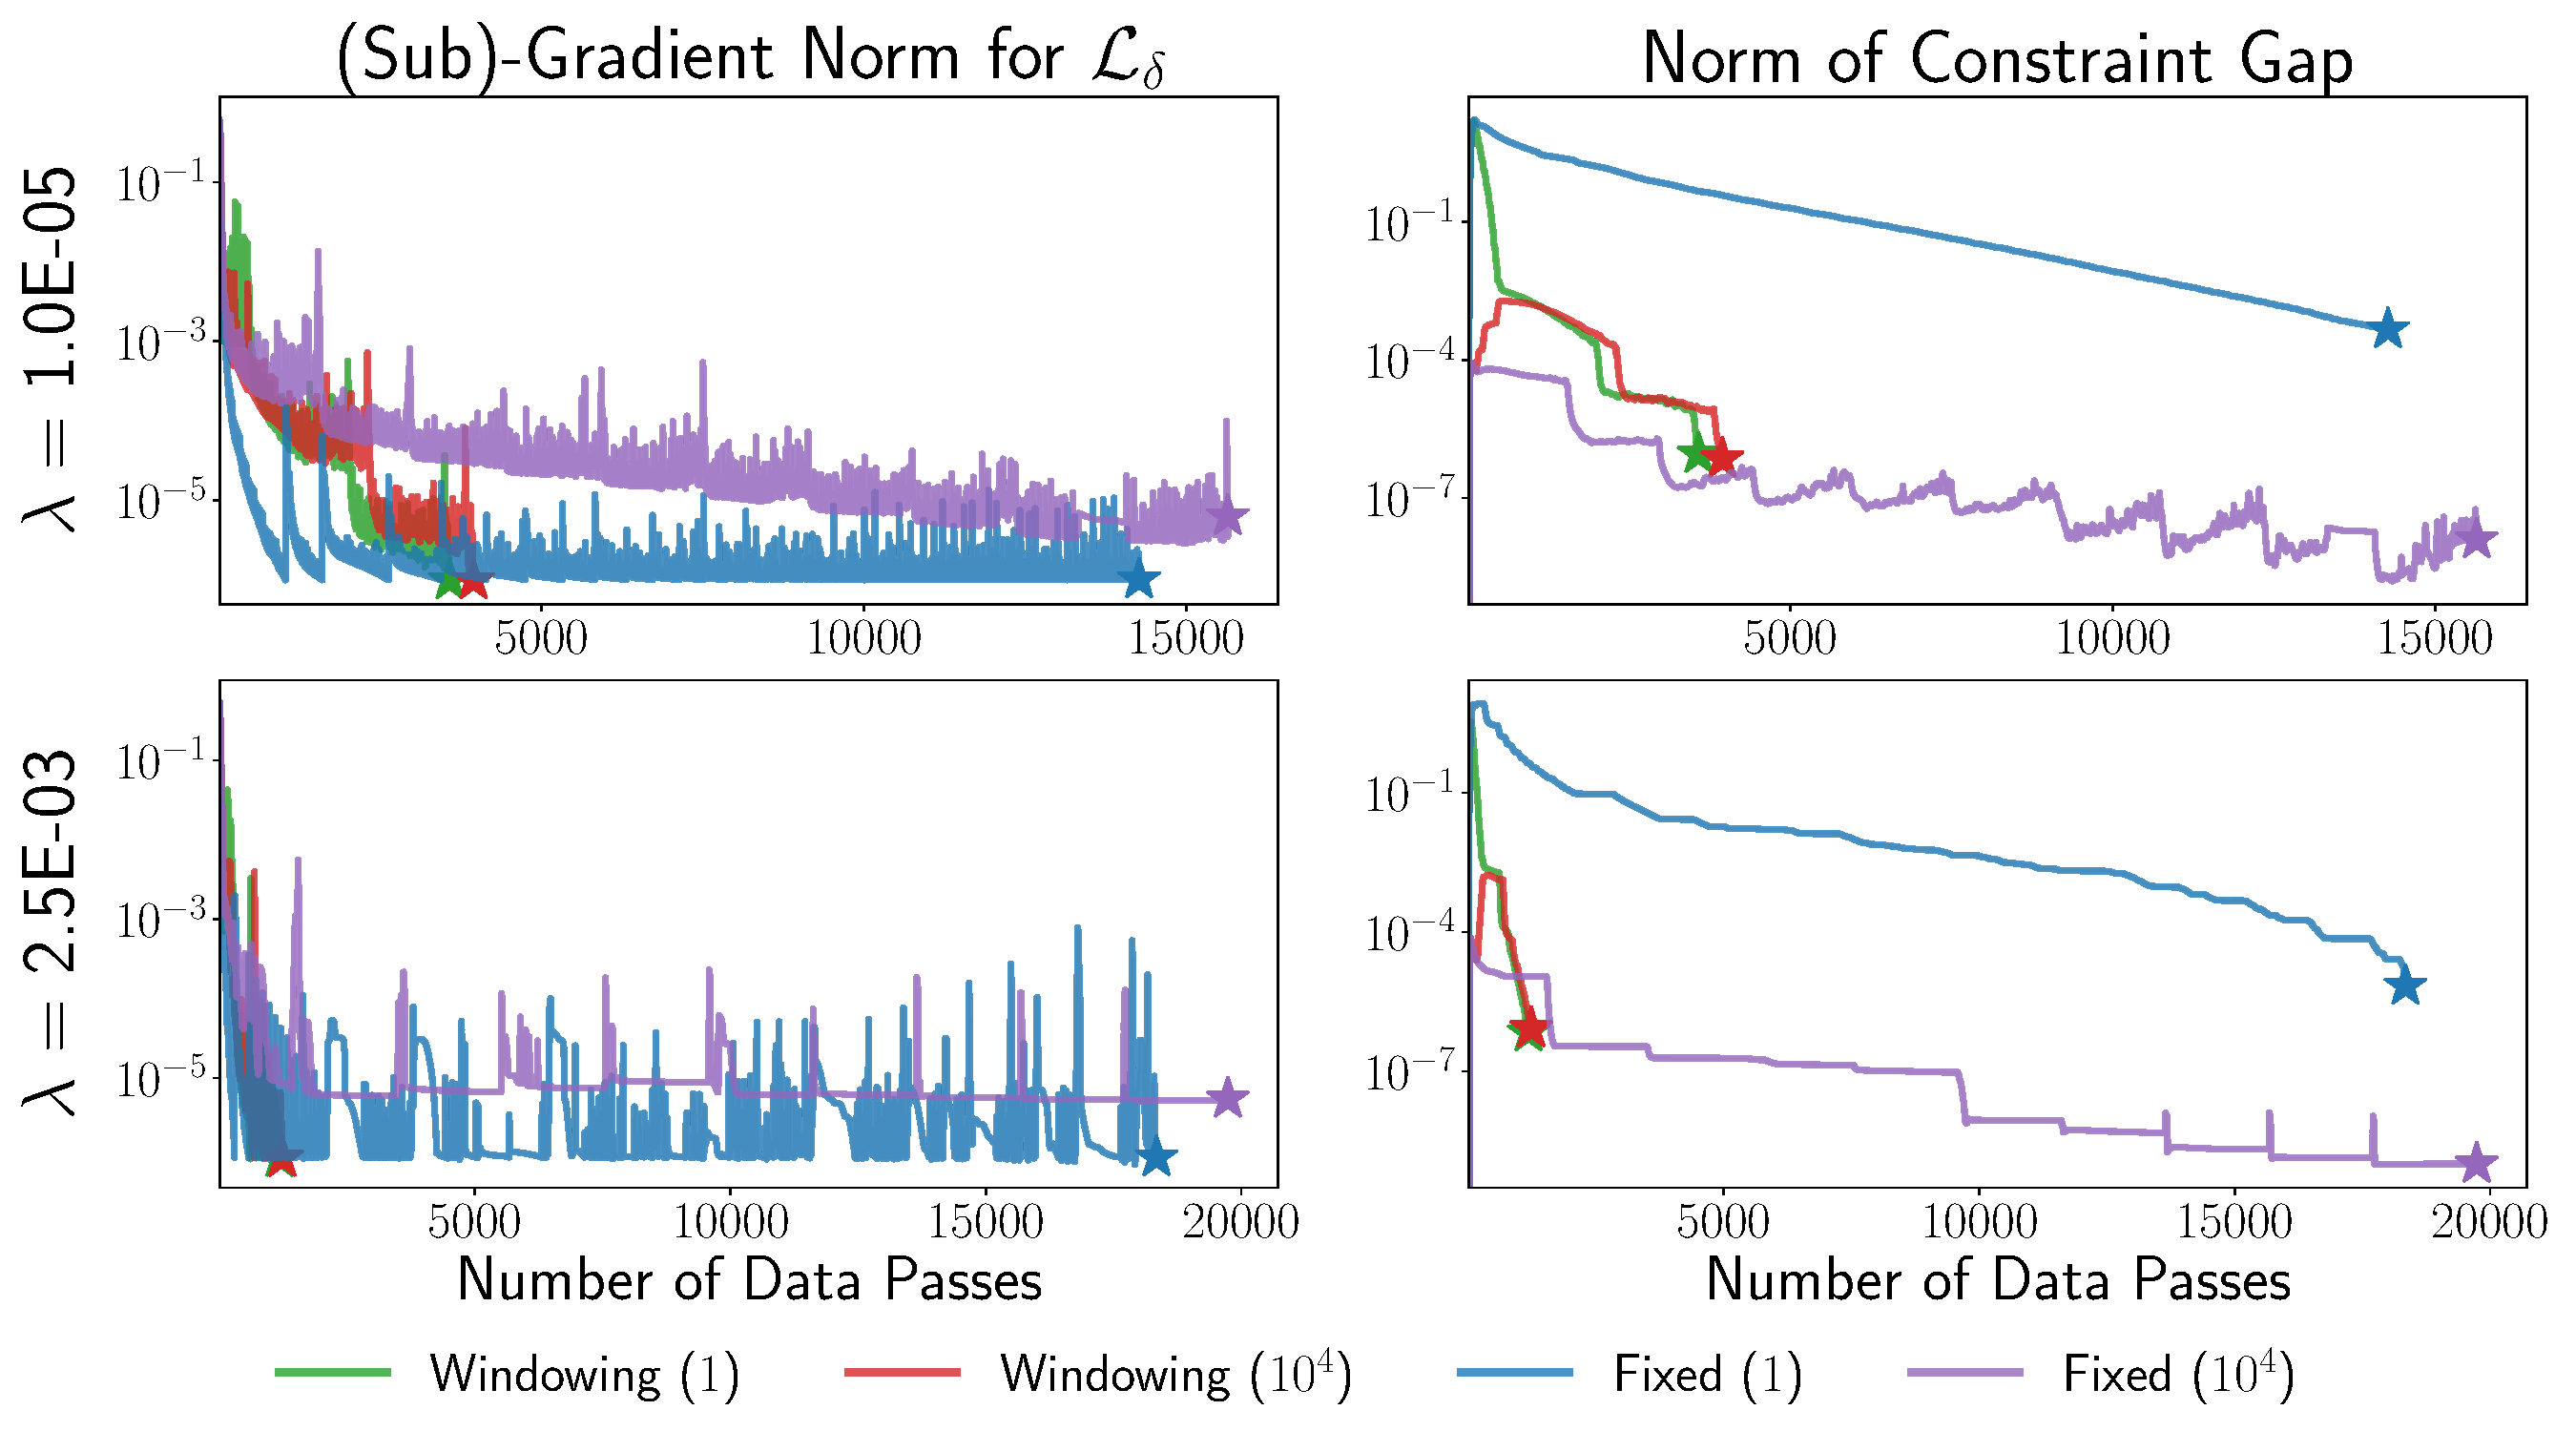
\includegraphics[width=0.95\linewidth]{figures/chapter_two/delta_heuristic/monks-2.pdf}
	\fi
	\caption{Convergence comparison for our AL method with with and without the windowing heuristic on the \texttt{monks-2} dataset.
		We show two extreme values of \( \delta \) (shown in parentheses) to illustrate failure models the AL method without our heuristic.
		Roughly, each ``bump'' in the subgradient norm (squared) of \( \calL_\delta \) corresponds to one prox-point iteration on the dual parameters (i.e.\ an AL update).
		Observe that when \( \delta \) is small, R-FISTA solves sub-problem~\eqref{eq:al-subroutine} quickly, but the AL method cannot find a feasible solution without an extreme number of dual updates.
		In contrast, R-FISTA never solves~\eqref{eq:al-subroutine} to the first-order tolerance (\( 10^{-6} \))  when \( \delta \) is very large.
		In this case, dual updates are triggered only by a limit on the number of R-FISTA iterations for solving the sub-problem. See Appendix~\ref{app:default-parameters}.
		The windowing heuristic corrects both failure modes.
	}%
	\label{fig:delta-heuristic-monks}
\end{figure}

\begin{figure}
	\centering
	\ifdefined\smallPDF
		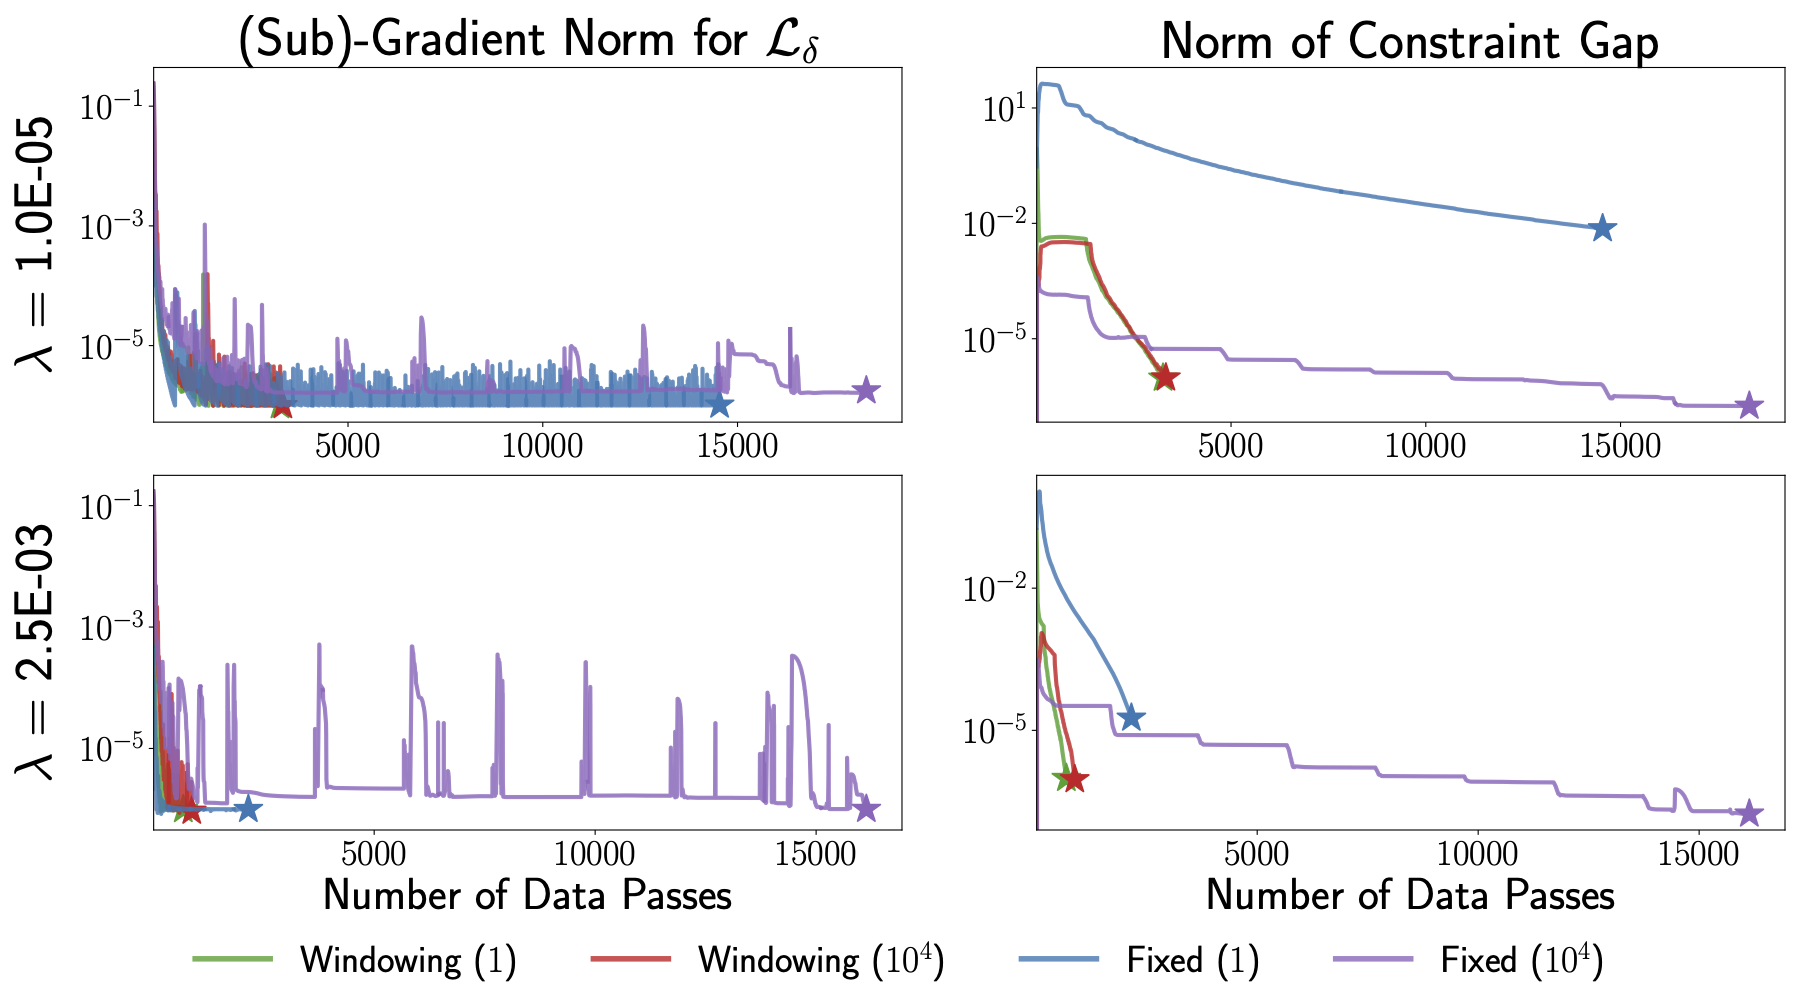
\includegraphics[width=0.95\linewidth]{figures/chapter_two/delta_heuristic/ilpd-indian-liver.png}
	\else
		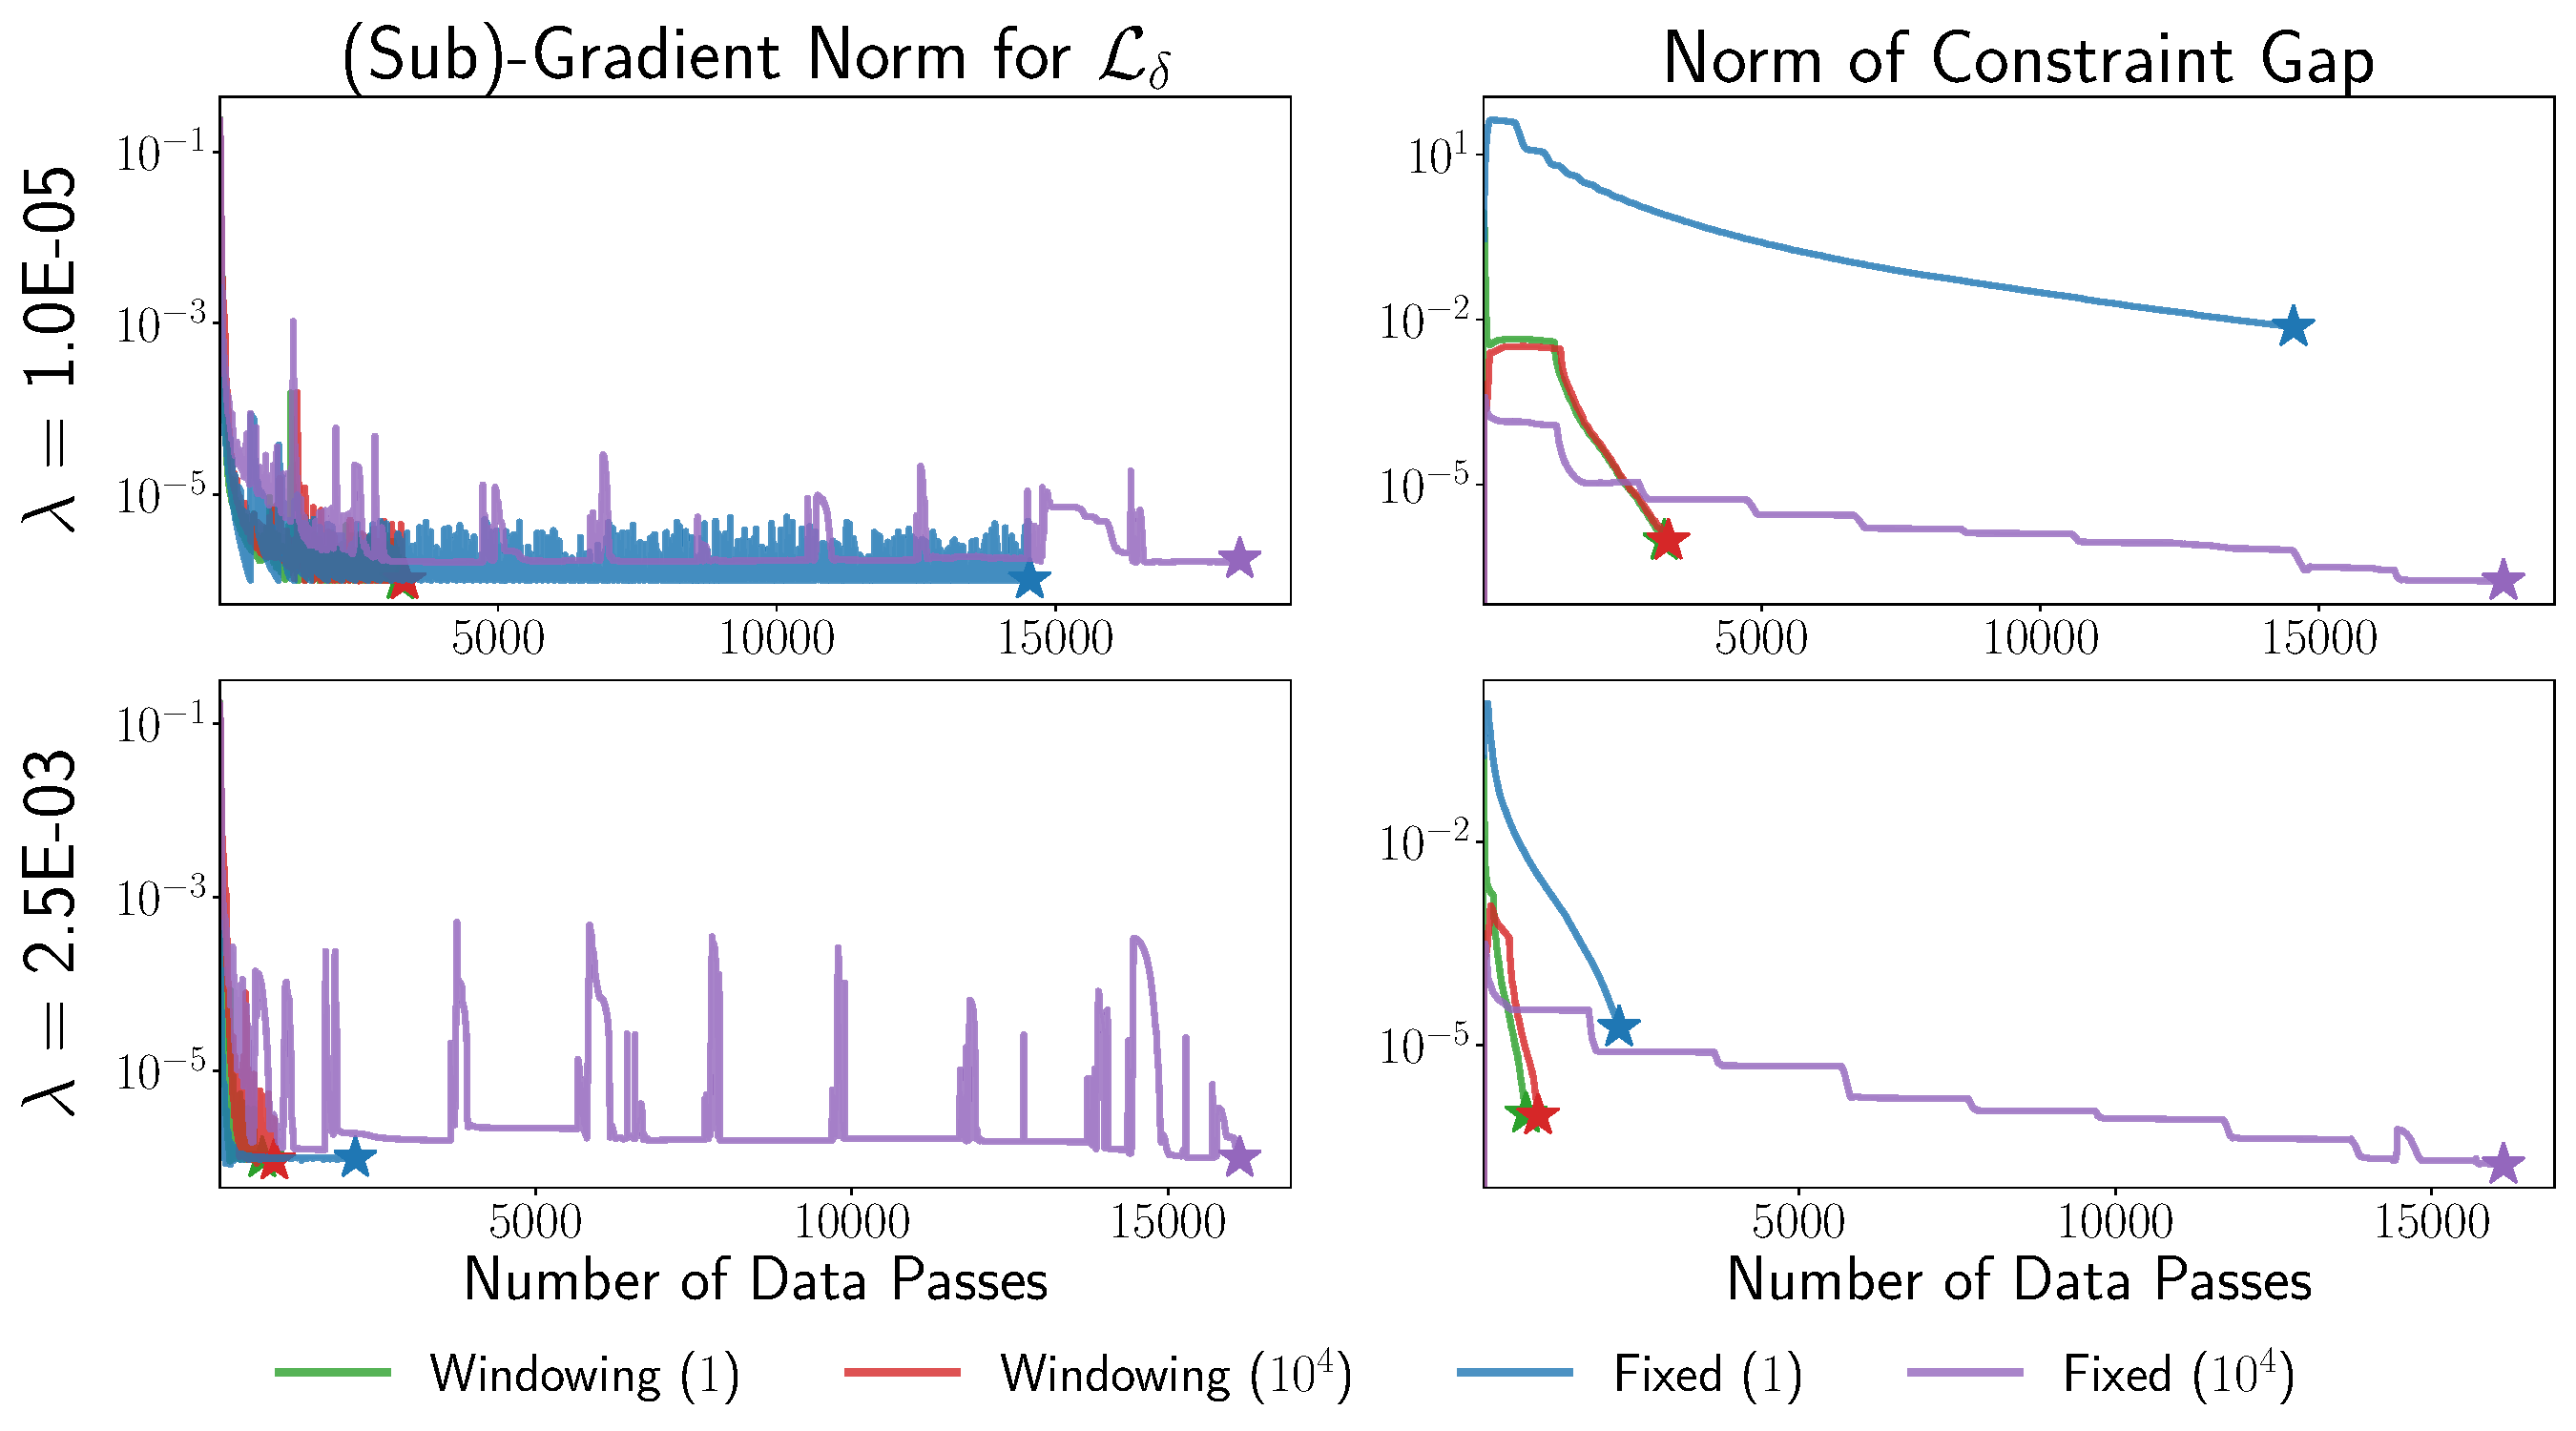
\includegraphics[width=0.95\linewidth]{figures/chapter_two/delta_heuristic/ilpd-indian-liver.pdf}
	\fi
	\caption{Convergence comparison for our AL method with with and without the windowing heuristic on the \texttt{ilpd-indian-liver} dataset.
		Penalty parameters \( \delta \) are reported in parenthesis. }%
	\label{fig:delta-heuristic-ilpd-indian-liver}
\end{figure}

We also provide convergence plots on two randomly selected datasets to better illustrate the failures modes of the AL method with miss-specified penalty strength.
Figures~\ref{fig:delta-heuristic-monks} and~\ref{fig:delta-heuristic-ilpd-indian-liver} and show detailed results for the \texttt{monks-2} and \texttt{ilpd-indian-liver} datasets.
When \( \delta \) is too small, the AL method easily solves subproblem~\eqref{eq:al-subroutine}, but struggles to make progress on the constraint gaps.
Intuitively, the step-size for the dual proximal-point algorithm is too small and a very large number of iterations is required to make progress on the dual problem.
Conversely, the augmented Lagrangian \( \calL_\delta \) is poorly conditioned when \( \delta \) is overly large and R-FISTA struggles to solve the primal sub-problem to the necessary tolerance.
The windowing heuristic corrects for both pathologies by ensuring the initial constraint gap is in a ``normal'' regime that balances penalizing constraint violations and conditioning of the subproblem.
This behavior is particularly noticeable for \texttt{monks-2}, where the windowing heuristic adjusts \( \delta \) to shrink the constraint gap (\( \delta = 1 \)) or relax the optimization problem (\( \delta = 10^4 \)).
